\documentclass[11pt]{article}
\usepackage{fullpage}
\usepackage{amsmath}
\usepackage{amssymb}
\usepackage{color}
\usepackage{framed}
\usepackage{graphicx}
\usepackage{float}
\usepackage{forest}
\usepackage{algorithm}
\usepackage{enumitem}
\usepackage[noend]{algpseudocode}

\renewcommand{\labelenumi}{\alph{enumi}.}
\begin{document}
\begin{center}
\begin{tabular*}{6.44in}{l @{\extracolsep{\fill}}c r}
	\bfseries  &  & \bfseries CSCI 3104: Algorithms\\
	\bfseries & & \bfseries Spring 2022 \\
	\bfseries&  & \bfseries  Recitation \#1 - Induction \\
\end{tabular*}
\end{center}

\begin{center}
	\noindent\textcolor{red}{\textbf{SOLUTIONS}}
\end{center}

\subsection*{Learning Objectives}
\begin{itemize}
\item know the parts of an inductive proof
\item use induction to prove facts about trees
\item identify errors in inductive proofs
\end{itemize}


%~~~~~~~~~~ PROBLEM 1 ~~~~~~~~~~

\subsection*{Problem 1}
Your friend excitedly shows you her proof that, for all $n\geq 1$, $\sum_{i = 1}^n (4i-3) = n(2n-1)$. She tells you that she's pretty sure she's gotten it right. Find any errors in your friend's proof and explain why each is incorrect. You don't need to write a corrected version, only explain the errors.

\begin{itemize}
	\item[]\textbf{Base Case.} Let $k = 1$. Then, $\sum_{i = 1}^k (4i-3) = 4\cdot 1 - 3 = 1$, and $k(2k-1) = 1(2\cdot 1 - 1) = 1$, and the statement holds.
	\item[]\textbf{Inductive Hypothesis.} Assume the statement holds for all $k\geq 1$.
	\item[]\textbf{Inductive Step.} We show it also holds for $k+1$. By the IH,
\begin{align}
	\sum_{i = 1}^{k+1} (4i-3) &= (k+1)(2(k+1)-1),
\end{align}
so we can conclude that
\begin{align}
	\sum_{i=1}^{k}(4i-3) &= k(2k-1) - (4(k+1) - 3)\\
	\sum_{i = 1}^{k} (4i-3) &= k(2k-1)
\end{align}
as claimed.
\end{itemize}
\begin{framed}
\noindent \textbf{SOLUTION.}
There are several errors here:
\begin{itemize}
	\item Your friend's IH assumes the statement holds \textbf{for all $k\geq 1$}, which simply assumes the claim is true and uses the claim to prove itself.
	\item In the IS, your friend has worked both sides of the equation, which can lead to incorrect results
	\item In the IS, your friend is working in the wrong direction from the base case even given a correctly stated IH. Say the IH were that the statement holds for $k + 1 \geq 1$. We cannot take the first step to expand which values we know this works for: at $k + 1 = 1$, our IS shows that this holds for $ k = 0$, but not for $k = 1$, the direction we are interested in showing.
	\item You might consider encouraging you friend to explain her work in the IS more thoroughly
\end{itemize}

\noindent A correct proof might be the following:
\begin{itemize}
	\item[]\textbf{Base Case.} Let $k = 1$. Then, $\sum_{i = 1}^k (4i-3) = 4\cdot 1 - 3 = 1$, and $k(2k-1) = 1(2\cdot 1 - 1) = 1$, and the statement holds.
	\item[]\textbf{Inductive Hypothesis.} Assume the statement holds for some $k\geq 1$.
	\item[]\textbf{Inductive Step.} We show it also then holds for $k+1$. We write the LHS of the $k +1$st case:
	\begin{align}
		\sum_{i = 1}^{k + 1} (4i-3)  &= \sum_{i = 1}^{k} (4i-3) + 4(k + 1)-3\label{pre_IH}\\
		&= k(2k-1) + 4k + 1\label{IH_applied}\\
		&= 2k^2 + 3k +1\\
		&= (k+1)(2k+1) = (k+1)(2(k+1) - 1),
	\end{align}
	where the IH is used to obtain equation (\ref{IH_applied}) from (\ref{pre_IH}).
\end{itemize}
\end{framed}
\newpage


%~~~~~~~~~~ PROBLEM 2 ~~~~~~~~~~

\subsection*{Problem 2}
\noindent\textbf{Definition 1.} The \emph{complete, balanced binary tree} of depth $d$ for $d\in \mathbb{N}$, denoted $\mathcal{T}(d)$, is defined as follows:
\begin{itemize}
	\item $\mathcal{T}(0)$ is a single vertex
	\item for $d > 0$, $\mathcal{T}(d)$ is a root vertex with two children, each the root of $\mathcal{T}(d-1)$.
\end{itemize}
For example:
\begin{center}
	\begin{forest}
		for tree={
			circle,
			draw,
			fill,
			minimum width=2pt, % size
			inner sep=0pt,
			parent anchor=center,
			child anchor=center,
			s sep+=25pt, % distance between children
		}
		[ ]
	\end{forest}
	\noindent \\ $\mathcal{T}(0)$.
\end{center}
\noindent \\
\begin{center}
	\begin{forest}
		for tree={
			circle,
			draw,
			fill,
			minimum width=2pt, % size
			inner sep=0pt,
			parent anchor=center,
			child anchor=center,
			s sep+=25pt, % distance between children
		}
		[ [] [] ]
	\end{forest}
	\noindent \\ $\mathcal{T}(1)$.
\end{center}
\noindent \\
\begin{center}
	\begin{forest}
		for tree={
			circle,
			draw,
			fill,
			minimum width=2pt, % size
			inner sep=0pt,
			parent anchor=center,
			child anchor=center,
			s sep+=25pt, % distance between children
		}
		[ [[][]] [[][]] ]
	\end{forest}
	\noindent \\ $\mathcal{T}(2)$.
\end{center}
\noindent Using induction, show that the tree $\mathcal{T}(d)$ has exactly $2^d - 1$ non-leaf nodes.
\begin{enumerate}
	\item State your induction variable and base case. Show that your base case is correct.
	\item State your inductive hypothesis.
	\item State your goal for the inductive step. Prove your inductive step. Where did you use your inductive hypothesis?
\end{enumerate}
\begin{framed}
	\noindent\textbf{SOLUTION.}
	Let $v_d$ denote the number of non-leaf vertices in the tree $\mathcal{T}(d)$.
	\begin{enumerate}
		\item We induct on the depth of the tree $d$, with base case $d = 0$. In this case, $v_0 = 0$ since there are no non-leaf nodes, and $2^0-1=0$, so the claim holds.
		\item Assume the claim holds for some fixed $d \geq 0$, and $v_d = 2^d -1$.
		\item We want to show that, if the claim holds for $\mathcal{T}(d)$, then the claim also holds for $\mathcal{T}(d+1)$, and $v_{d+1} = 2^{d+1}-1$.

		Firstly, note that $v_{d+1} = 2v_d + 1$, since $\mathcal{T}(d+1)$ has all the non-leaf vertices of two trees $\mathcal{T}(d)$, plus a new root (non-leaf) vertex, and all leaf vertices in the subtrees $\mathcal{T}(d)$ are still leaves. Then,
		\begin{align}
			v_{d+1} &= 2v_d + 1 \label{pre_IH_2}\\
			&= 2\left(2^d - 1\right) + 1\label{IH_applied_2}\\
			&= 2^{d+1} - 2 + 1 = 2^{d+1} - 1,
		\end{align}
		where the IH gives us that line (\ref{pre_IH_2}) can be written as (\ref{IH_applied_2}).
	\end{enumerate}
\end{framed}
\newpage


%~~~~~~~~~~ PROBLEM 3 ~~~~~~~~~~

\subsection*{Problem 3}
Recall \textproc{Mergesort}, which sorts an array $A[1, \ldots, n]$ (here, the notation $A[1, \ldots, n]$ indicates an array of length $n$ with indices $1, \ldots, n$). \textproc{Mergesort} recursively sorts $A[1, \ldots, n/2]$ and $A[n/2+1, \ldots, n]$, and then merges the two sorted sub-arrays into a single sorted array. Pseudocode for \textproc{Mergesort} is below. You may assume the \textproc{Merge} function correctly merges the two sorted sub-arrays into a single sorted array. The goal of this problem is to prove the correctness of \textproc{Mergesort} by induction.

\begin{enumerate}
	\item Clearly identify the base case(s). Why does \textproc{Mergesort} correctly sort arrays in these cases?
	\item Formulate an inductive hypothesis. [\textbf{Note:} Will you want to use a weak inductive hypothesis or strong inductive hypothesis? Try to answer this question and explain your reasoning. Don't hesitate to talk with your classmates or TA if you get stuck!]

	\item We now consider the inductive step.
	\begin{enumerate}[label = \roman*.]
		\item What are the smaller cases that we need to consider? Why?
		\item How do we know that \textproc{Mergesort} correctly sorts these smaller cases?
		\item Once \textproc{Mergesort} sorts these smaller cases, how do we know that \textproc{Mergesort} correctly sorts $A[1, \ldots, n]$, the original input array?
	\end{enumerate}

	\item Using your work in parts (a)-(c), write a proof of correctness for \textproc{Mergesort}.
\end{enumerate}

\begin{algorithm}
	\caption{Mergesort}\label{alg:Mergesort}
	\begin{algorithmic}[1]
		\Procedure{Mergesort}{$\text{Array} A[1, \ldots, n]$}

		\If{$\text{len(A)} \leq 1$}
		\Return A
		\EndIf

		\State $\text{Left} \gets []$
		\State $\text{Right} \gets []$ \\

		\For{$i \gets 1; i \leq \text{len}(A)/2; i \gets i+1$}
		\State $\text{Left}[i] \gets A[i]$ \\
		\EndFor

		\For{$i \gets \text{len}(A)/2 + 1, j \gets 1; i \leq \text{len}(A); i \gets i+1, j \gets j +1$}
		\State $\text{Right}[j] \gets A[i]$ \\
		\EndFor

		\State \text{Mergesort}(\text{Left})
		\State \text{Mergesort}(\text{Right})
		\State \text{Merge}(Left, Right, A)
		\EndProcedure
	\end{algorithmic}
\end{algorithm}
\begin{framed}
\noindent\textbf{SOLUTION.}

\begin{enumerate}
	\item The base cases are when $n = 0, 1$. Here, \textproc{Mergesort} returns the array. Note that an array of length $n = 0$ or $n = 1$ is already sorted--there is no additional work that needs to be done.

	\item Fix $k \geq 1$. Suppose that \textproc{Mergesort} correctly sorts any array of length at most $k$. This is \emph{strong induction}, since we assume \textproc{Mergesort} correctly sorts anything of length $\leq k$ rather than of lenfth exactly $k$. \\

	Strong induction is necessary here because \textproc{Mergesort} on an array of length $n$ requires that \textproc{Mergesort} be able to successfully sort lists of length approximately $n/2$, not $n-1$.

	\item We now consider the inductive step.
	\begin{enumerate}[label=\roman*.]
		\item \textproc{Mergesort} recursively sorts the \texttt{Left} and \texttt{Right} sub-arrays. Therefore, these are the two smaller cases we need to consider, each of size approximately $n/2$ (rounded up and down, since if $n$ is not even one list will take the extra element).


		\item \textproc{Mergesort} correctly sorts these smaller cases because \texttt{Left} and \texttt{Right} have fewer than $k$ elements. By the inductive hypothesis, \textproc{Mergesort} correctly sorts both \texttt{Left} and \texttt{Right}.

		\item Once \textproc{Mergesort} sorts these smaller cases, how do we know that \textproc{Mergesort} correctly sorts $A[1, \ldots, n]$, the original input array?

			By assumption in the problem statement, the \textproc{Merge} function correctly merges the two sorted sub-arrays into a single sorted array.
	\end{enumerate}
	\item Using your work in parts (a)-(c), write a proof of correctness for \textproc{Mergesort}.
	We prove by induction on $n \in \mathbb{N}$ the length of the input array $A$, that \textproc{Mergesort} correctly sorts the input array.
	\begin{itemize}[label=]
		\item \textbf{Base Cases:} We consider the cases when $n = 0, 1$. Note that an array of length $n \leq 1$ is already sorted, and so there is no more work to be done. In these cases, \textproc{Mergesort} (at line 2) returns $A$ and terminates.

		\item \textbf{Inductive Hypothesis:} Fix $k \geq 1$. Suppose that \textproc{Mergesort} correctly sorts any array of length at most $k$.

		\item \textbf{Inductive Step:} Suppose $A[1, \ldots, k+1]$ is an array of length $k+1$. At lines 3-10, \textproc{Mergesort} constructs arrays \texttt{Left} and \texttt{Right}, where the elements of $A[1, \ldots, (k+1)/2]$ are copied into \texttt{Left} in the order they appear in $A$, and the elements of $A[(k+1)/2, \ldots, k+1]$ are copied into \texttt{Right} in the order they appear.

		Now at lines 12 and 13, \textproc{Mergesort} recursively invokes itself, passing \texttt{Left} and \texttt{Right}, respectively. As \texttt{Left} and \texttt{Right} have length less than $k$, we have by the inductive hypothesis that \textproc{Mergesort} correctly sorts both \texttt{Left} and \texttt{Right}. So at Line 14, both \texttt{Left} and \texttt{Right} are sorted. Therefore, by assumption, \textproc{Merge} correctly merges \texttt{Left} and \texttt{Right} back into $A$, so that $A$ is sorted.
	\end{itemize}

	The result follows by induction.
	\end{enumerate}
\end{framed}
\newpage

%~~~~~~~~~~ PROBLEM 4 ~~~~~~~~~~

\subsection*{Problem 4 (Bonus)}
The puzzle game the Tower of Hanoi consists of three upright pegs, and $n$ disks of different diameters which fit over the pegs. The puzzle starts with the disks all stacked on the first peg, with the largest diameter on the bottom decreasing in size to the smallest disk on top, as follows:
\begin{figure}[H]
	\begin{center}
		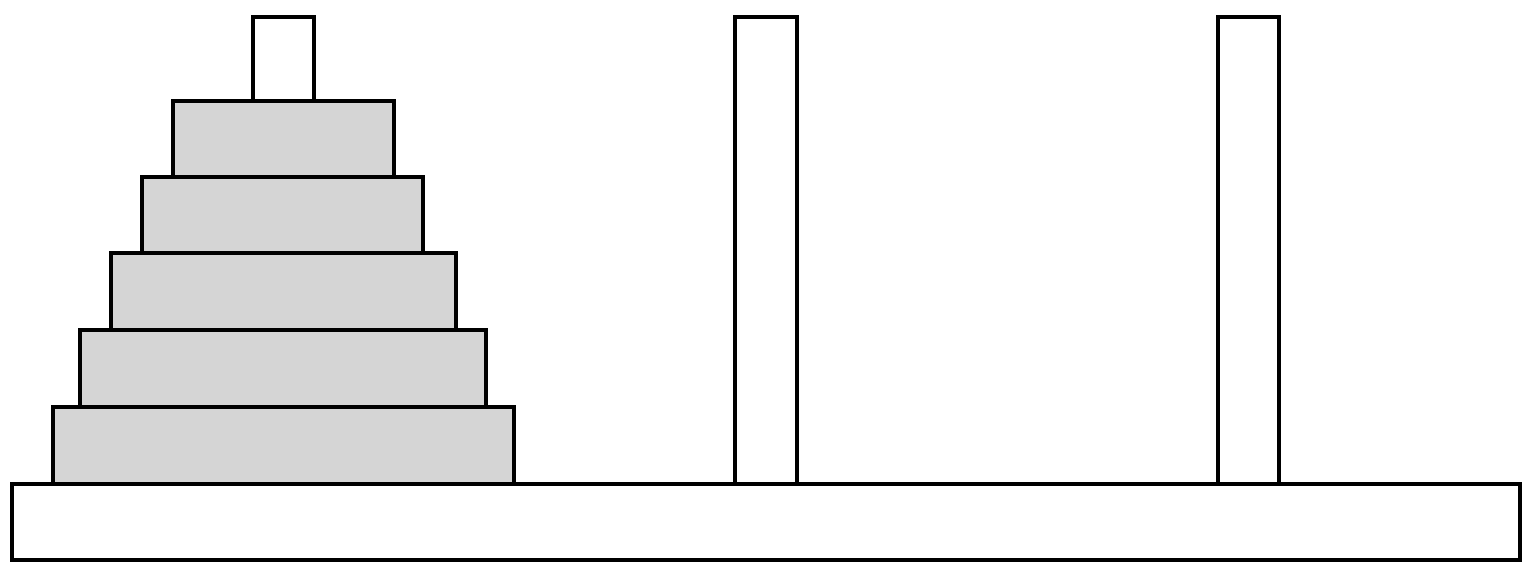
\includegraphics[height=4cm]{hanoi.png}
	\end{center}
\end{figure}
The objective of the puzzle is to transfer this ``pyramid'' to the third peg in the same configuration: largest disk on the bottom up to the smallest on top. Each move consists of moving a single disk from its current peg to a different peg, and disks can only be placed onto either an empty peg or a disk of a larger diameter. \\

Use induction to show that a Tower of Hanoi with $n$ disks can be solved in $2^n-1$ moves. \\

(hint: without loss of generality, if you can move the tower to the third peg in $k$ moves, you can also move the tower to the second peg in $k$ moves)

\begin{framed}
	\noindent\textbf{SOLUTION.} We can generalize the problem to be the number of moves to move a tower of $n$ disks to any peg, starting from any peg, assuming there are no smaller disks on either other peg.

	We induct on $n$, the number of disks. Let $x_n$ denote the number of moves it takes to move an $n$-disk tower to a different peg.
	\begin{itemize}
		\item[]\textbf{Base Case.} When $n = 1$, we can simply pick up the entire tower and move it to the desired peg in one move. Since $2^1 - 1 = 1$, the claim holds.
		\item[]\textbf{Inductive Hypothesis.} Assume that the claim holds for some fixed height of $n\geq 1$ disks.
		\item[]\textbf{Inductive Step.}  We show we can also move a tower of height $n+1$ disks to peg 3 in $2^{n+1} - 1$ moves.

		Since we can move a tower of $n$ disks to another peg in $v_n = 2^n-1$ moves, we can move the top $n$ disks to the second peg, move the $n+1$st disk to the third peg, and then move the $n-$-disk stack on top of our $n+1$st peg to move the whole tower. Thus, the complete tower can be moved to a different peg in
		\begin{align*}
			v_{n+1} &= v_n + 1 + v_n\\
			&= 2^n - 1 + 1 + 2^n - 1\\
			&= 2(2^n) - 1\\
			&= 2^{n+1} - 1
		\end{align*}
		moves, as claimed.
	\end{itemize}
\end{framed}
\end{document}
